\section{Agent Learning Speed Doubles Approximately Every Three Months}
\label{sec:scaling}

Frontier agents can now improve through interaction with task environments. This
raises a separate question: are newer models learning from their
environments faster? We measure this by comparing how much performance each
agent gains over a fixed interaction budget across model release dates.

\subsection{Experimental Design}
\label{sec:measuring}

\underline{\textit{Disentangling prior knowledge from environment learning.}}
A high score may reflect what the model already knew rather than what it learned during the run. To reduce this confound, we select an 18-task slice from \benchmark{} where models show similar first-attempt performance. With comparable starting points, later gains provide a cleaner measure of environment learning. We measure task-learning speed as the \textbf{average performance gain} over a fixed two-hour budget.

\underline{\textit{Evaluation protocol.}}
We evaluate frontier open- and closed-source AI systems released from September 2025 through the current evaluation window, when frontier systems became capable of sustained autonomous runs. Each model is run three times per task. GPT models are run with Codex; all other models are run with Claude Code. As shown in Figure~\ref{fig:performance-effort} (left), models start from comparable first-attempt performance on this 18-task slice, with an average of $6.87 \pm 0.97$.


\begin{figure}[!t]
\centering
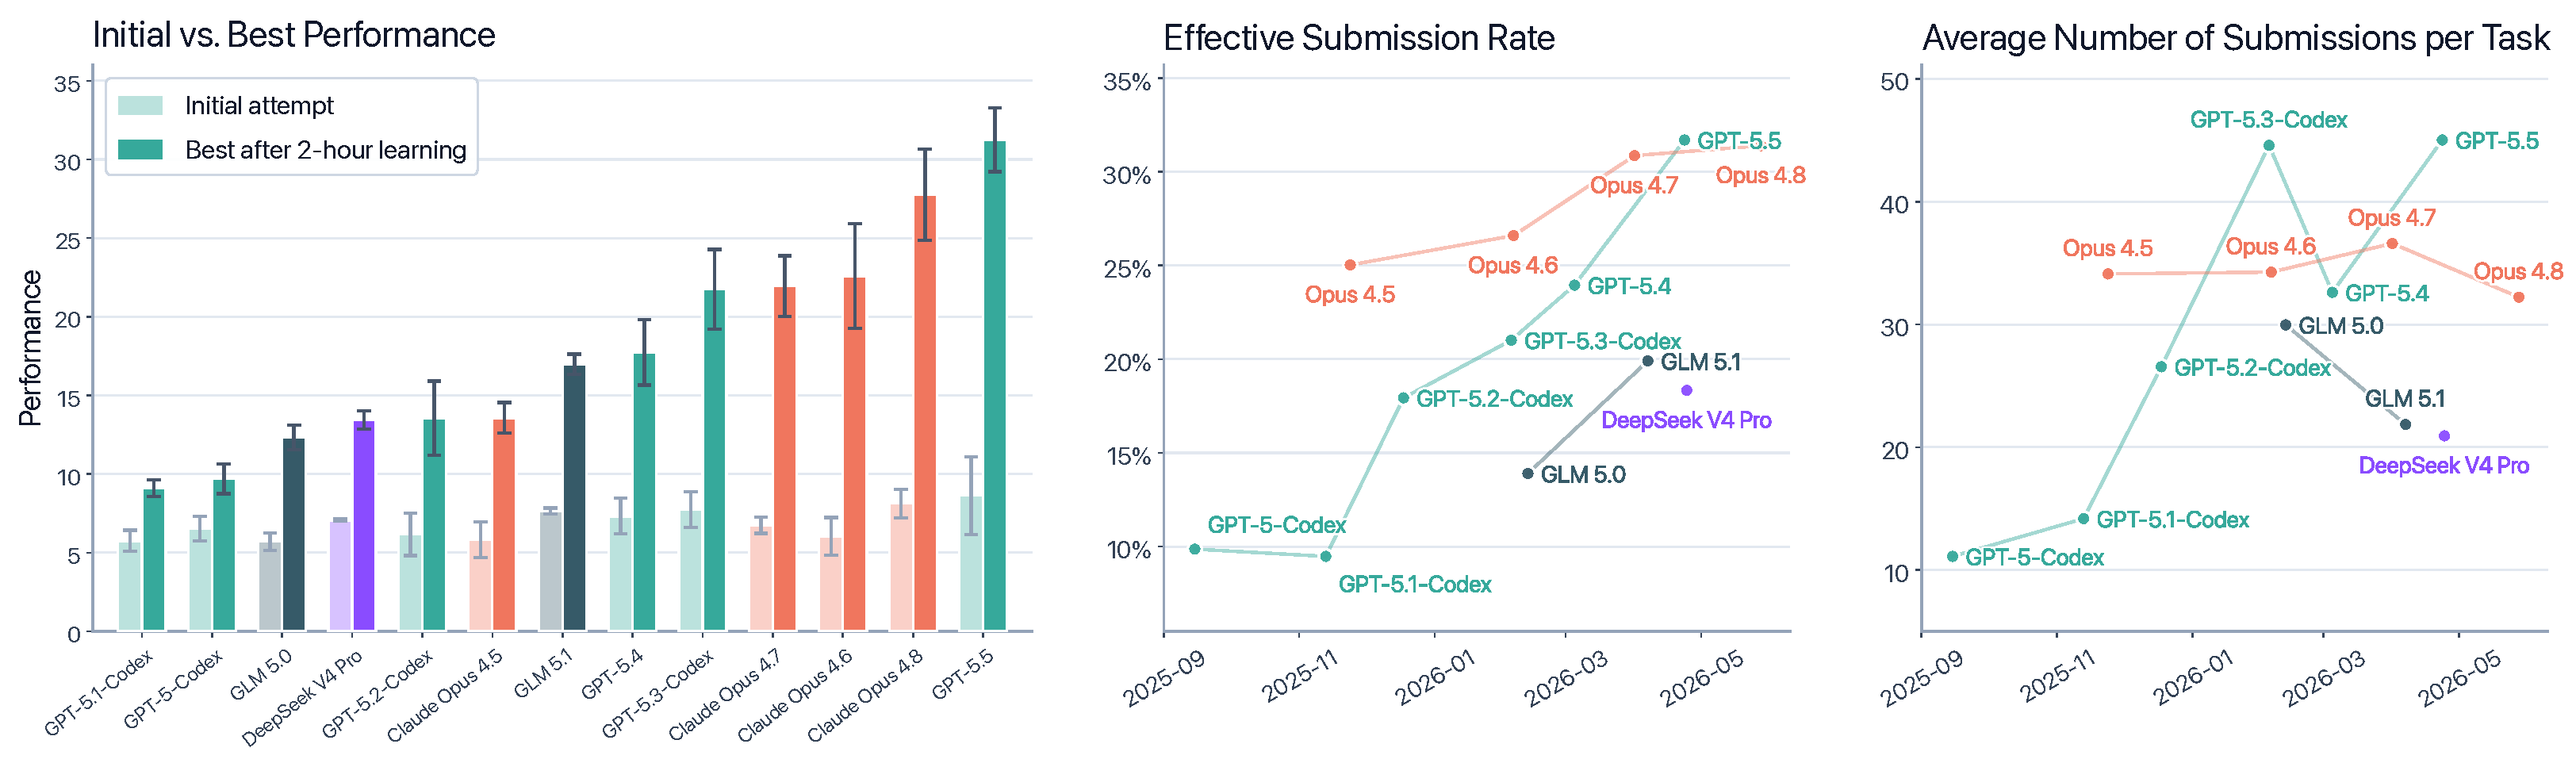
\includegraphics[width=\linewidth]{figures/performance_effort_combo_agent_initial_row.pdf}
\caption{Learning outcomes and agent effort on the 18-task slice. Left: normalized initial performance and best performance after two hours. Middle: fraction of submissions that improve the best-so-far score. Right: average number of submissions per task. Error bars in the left panel show uncertainty over three replicate runs.}
\label{fig:performance-effort}
\end{figure}

\subsection{Learning Speed across Model Generations}

Figure~\ref{fig:scaling} reports the two-hour evaluation results on the fixed 18-task slice. The y-axis measures agent learning speed, defined as performance gain over two hours, on a log scale. To estimate the frontier trend, we use darker markers to highlight the top two models at each release date. We then fit a linear trend to these frontier points, with the fitted 95\% confidence interval shown as the shaded band.

Figure~\ref{fig:scaling} shows a rapid increase in learning speed across recent model generations. From GPT-5-Codex in September 2025 to GPT-5.5 in April 2026, learning speed increases by roughly $8\times$ over 221 days. A log-linear fit to the frontier models captures this trend well, corresponding to \textbf{an approximate doubling every three months}. Figure~\ref{fig:performance-effort} shows that this improvement is not simply explained by more frequent submissions. Submission frequency (right panel) changes unevenly: newer GPT models submit more actively, while other families do not. The middle panel tells a different story: later models turn a larger fraction of submissions into best-so-far improvements. This trend therefore reflects more effective learning from each interaction, not merely more attempts.
